\documentclass[11pt]{beamer}
\usetheme{metropolis}
%\usetheme{Warsaw}
%\usecolortheme{crane}
\usepackage[utf8]{inputenc}
\usepackage{amsmath}
\usepackage{amsfonts}
\usepackage{amssymb}
\usepackage{graphicx}
\usepackage{tikz}
\usetikzlibrary{shapes}
\usetikzlibrary{arrows}
\usepackage[czech]{babel}
\usepackage{pgfplots}
\usepackage{pgf}
\usepackage{hyperref}
\usepackage{multirow}
\usepackage{pdfpages}
\usepackage{subfigure}

\makeatletter
\setbeamertemplate{progress bar in head/foot}{
  \nointerlineskip
  \setlength{\metropolis@progressinheadfoot}{%
    \paperwidth * \ratio{\insertframenumber pt}{\inserttotalframenumber pt}%
  }%%
  \begin{beamercolorbox}[wd=\paperwidth]{progress bar in head/foot}
    \begin{tikzpicture}
      \draw[bg, fill=bg] (0,0) rectangle (\paperwidth, 2pt);
      \draw[fg, fill=fg] (0,0) rectangle (\metropolis@progressinheadfoot, 2pt);
    \end{tikzpicture}%
  \end{beamercolorbox}
}
\makeatother

\definecolor{theme-primary}{RGB}{0, 111, 186}
\definecolor{theme-secondary}{RGB}{255, 64, 64}

\author{Jan Vargovský}
\title{Black Friday dataset}
\subtitle{Metody analýzy dat III}
%\setbeamercovered{transparent} 
%\setbeamertemplate{navigation symbols}{} 
\institute{Katedra informatiky, FEI, VŠB-TU Ostrava}
\date{17. prosince 2018} 
%\logo{\pgfputat{\pgfxy(-1,6.5)}{\pgfbox[right,base]{\includegraphics[height=1.5cm,keepaspectratio]{logo-small}}}}

\graphicspath{ {figures/} }
\metroset{block=fill, numbering=fraction, progressbar=frametitle}
%\setbeamertemplate{section in toc}[sections numbered]
%\defbeamertemplate{frame numbering}{none}{}
%\setbeamertemplate{frame footer}{Jan Vargovský}
\setbeamercolor{palette primary}{bg=theme-primary}
%\setbeamertemplate{itemize items}{\small$\bullet$} 

\begin{document}

\begin{frame}
\titlepage
\end{frame}

\begin{frame}{Základní info}
\begin{itemize}
	\item Obsahuje \alert{537577} nákupů od \alert{5891} uživatelů.
	\item Každý zákazník má uvedeno:
		\begin{itemize}
			\item věkovou kategorii (7),
			\item pohlaví (2),
			\item kde žije (3),
			\item jak dlouho v daném místě žije (5),
			\item jestli je sám nebo s někým (2),
			\item a jaké má povolání (21).
		\end{itemize}
	\item Transakce pak obsahuje:
		\begin{itemize}
			\item ID výrobku (3623),
			\item 1 až 3 kategorie (18),
			\item a cenu ($185 - 23961$, $\mu=9333$, $\sigma=4981$).
		\end{itemize}	
	\item Dataset neobsahuje žádné chybějící data.	
\end{itemize}
\end{frame}

\begin{frame}{Distribuce zákazníků podle věkových kategorií}
\begin{figure}
	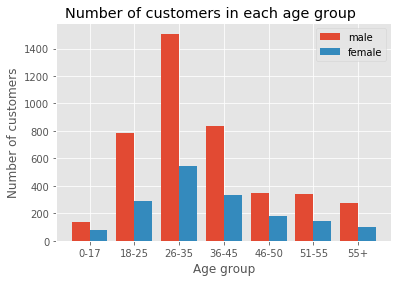
\includegraphics[width=0.7\textwidth,keepaspectratio]{black-friday_8_0}
\end{figure}
\end{frame}

\begin{frame}{Mužů je více a utratí více jak ženy}
\begin{figure}
	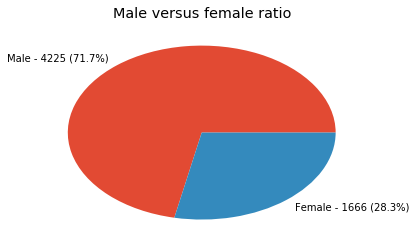
\includegraphics[width=0.5\textwidth,keepaspectratio]{black-friday_10_0}
\end{figure}
\begin{figure}
	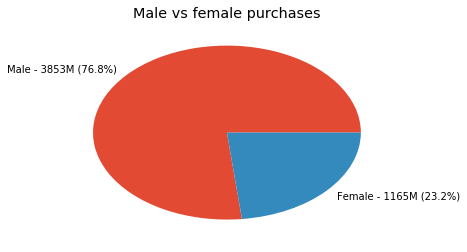
\includegraphics[width=0.5\textwidth,keepaspectratio]{black-friday_11_0}
\end{figure}
\end{frame}

\begin{frame}{Nejvíce se nakupují výrobky z 1., 5. a 8. kategorie}
\begin{figure}
	\hfill
	\subfigure[Počet]{
		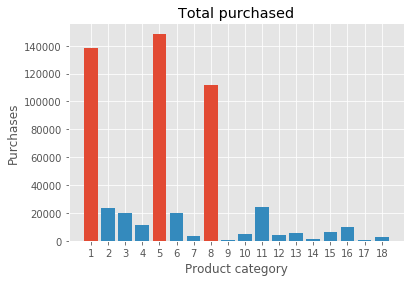
\includegraphics[width=0.45\textwidth,keepaspectratio]{black-friday_19_0}
	}
	\hfill
	\subfigure[Obrat]{
		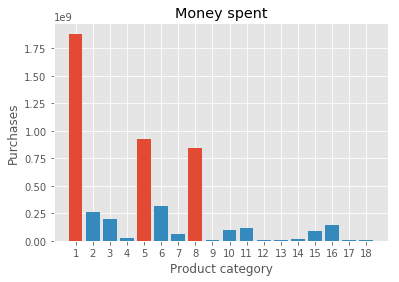
\includegraphics[width=0.45\textwidth,keepaspectratio]{black-friday_20_0}
	}
	\hfill
\end{figure}
\end{frame}

\begin{frame}{Čím starší jste, tím (pravděpodobně) více utratíte}
\begin{figure}
	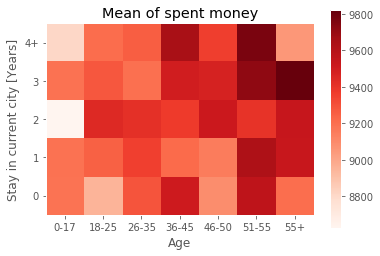
\includegraphics[width=0.7\textwidth,keepaspectratio]{black-friday_24_0}
\end{figure}
\end{frame}

\begin{frame}{Nejvíce se nakupuje ve městě B a v 2. roce co tam žijete}
\begin{figure}
	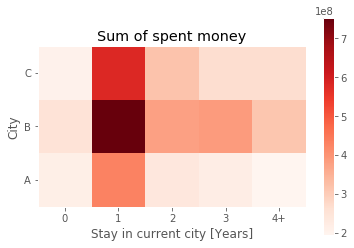
\includegraphics[width=0.7\textwidth,keepaspectratio]{black-friday_28_0}
\end{figure}
\end{frame}

\begin{frame}{Pravidlo 80/20 pro celkovou sumu nákupu}
\begin{figure}
	\hfill
	\subfigure{
		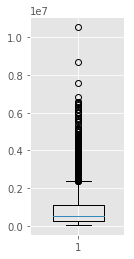
\includegraphics[width=0.3\textwidth,keepaspectratio]{black-friday_35_0}
	}
	\hfill
	\subfigure{
		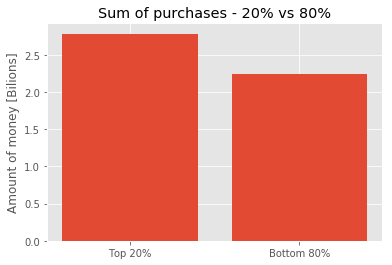
\includegraphics[width=0.6\textwidth,keepaspectratio]{black-friday_36_0}
	}
	\hfill
\end{figure}
\end{frame}

\begin{frame}{Odhad kolik zákazník utratí pomocí random forest}
\begin{figure}
	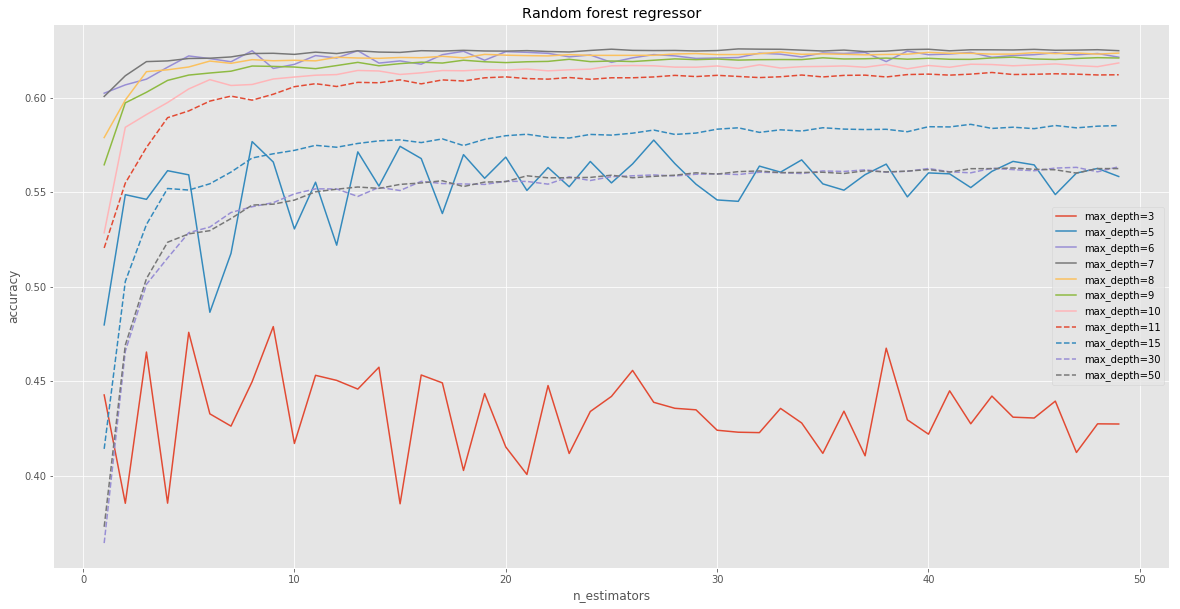
\includegraphics[width=\textwidth,keepaspectratio]{black-friday_43_0}
\end{figure}
\end{frame}

\begin{frame}
Dataset je dostupný zde: \url{https://www.kaggle.com/mehdidag/black-friday}
\end{frame}

\begin{frame}[standout]
Děkuji za pozornost
\end{frame}

\end{document}